\section{Abstraction via Super-Classes}

%-----------------------------------------------------------------------------------

\subsection{Thinking at Different Levels of Abstraction (Part 1)}

We think quite naturally at different levels of abstraction. Consider the sentence
Consider the following statements which become more and more concrete:

\vspace{2mm}
\centerline{\em A person deposited money into the account.}
\vspace{2mm}

\centerline{\em A client deposited money into the account.}
\vspace{2mm}

\centerline{\em Mr P.J. Smith deposited money into the account.}
\vspace{2mm}

It might be sufficient for you to know that somebody deposited money in the account.
Alternatvely, you might want to know whether it is a cient or a friend who deposited
the money and for bookkeeping purposes you would want to know which client deposited 
the money into the account. Here client is a special type of person, and P.J. Smith
may be a special kind of client.

So we naturally introduce abstractions into our everyday language and it is really in
the same spirit that object-oriented languages support abstraction too. 

%-----------------------------------------------------------------------------------

\subsection{Specialization through Subclassing \label{secSubClassing}}

Java allows you to define objects at various levels of abstraction. For example,
You might view a particular manager as a \verb+Manager+, an \verb+Employee+, a 
\verb+Person+ or simply as an \verb+Object+. This is a process from very concrete
to more and more abstract. 

The reverse direction can be viewed as specialization. A \verb+Manager+ {\em is 
a} special type of \verb+Employee+ which {\em is a} special type of \verb+Person+ 
which {\em is a} special type of \verb+Object+. 

Note that we can identify a {\em specialization relation} ship as a 
{\em is a special kind of}
relationship and this should \underline{\bf always} be the criterion for
deciding on subclassing.

Subclassing is achieved in via the following syntax:

\noindent{\small\begin{verbatim}
class Manager: public Employee {...};

class Employee: public Person {...};

class Person {...};
\end{verbatim}}

Here \verb+Manager+ is a {\em subclass} of \verb+Employee+ which is a subclass 
of \verb+Person+. Conversely, \verb+Person+ is the superclass of \verb+Employee+
which is the superclass of \verb+Manager+. Note that we did not have to specify
that \verb+Person+ extends Object. 

I want to stress that the language relies on you to design your class 
hierarchies in such a way that the subclass {\em is a} specialization of the 
superclass. This is best illustrated by the following simple statements:

\noindent{\small \begin{verbatim}
Employee* employee;

employee = new Manager();
\end{verbatim}}

We first declare a pointer to an \verb+Employee+. This pointer can refer to
any object which {\em is an} \verb+Employee+. In the second statement we create
a \verb+Manager+ and assign the \verb+Employee+-pointer to refer to the 
manager. The compiler is quite happy because \verb+Manager+ is a subclass of
\verb+Employee+ and he/she trusts you in having applied the {\em is a} criterion
for subclassing. 

Quite generally the following rule should hold. Everywhere where an 
\verb+Employee+ is required you should be able to supply any \verb+Employee+,
whether it is a vanilla \verb+Employee+ or a specialized \verb+Employee+
like \verb+Manager+ or \verb+Programmer+. We can thus work with employees
at various levels of abstraction. Let us have a look at the intestines of a 
simple \verb+Person+ class.

%---------------------------------

\subsubsection{The Person Header}

The \verb+Person+ class has no surprises with the exception of a 
\verb+toString()+ method which has been declared virtual. We shall
discuss this method in section \ref{secPolymorphism}.

\noindent {\small \input{Abstraction/Programs/Person.h}}

%---------------------------------

\subsubsection{The Person Implementation}

The implementation class is similarly straight-forward:

\noindent {\small \input{Abstraction/Programs/Person.cpp}}

%---------------------------------

\subsubsection{The Header for the Employee Sub-Class}

The \verb+Employee+ class is declared a subclass of the \verb+Person+
class via

\noindent{\small \begin{verbatim}
class Employee: public Person {...};
\end{verbatim}}

The subclass inherits all instance members -- not the class (\verb+static+)
members from the superclass. Hence, we do not define data fields for the 
name and id number. Note that these fields were
declared \verb+private+ in the \verb+Person+ class and that they thus
cannot be directly accessed from the subclass. They are still inherited,
though. If we want to acces them from the subclass, we have to use the 
same public interface as everybody else. 

With the name and id number inherited, we only have to define a data
field with corresponding query and set methods for the additional
\verb+salary+ field:

\noindent {\small \input{Abstraction/Programs/Employee1.h}}

%---------------------------------

\subsubsection{The Implementation File for the Employee Sub-Class}

When instantiating a class, one always instantiates all its superclasses.
For example, everytime an instance of the \verb+Employee+ class is created, 
an instance of the \verb+Person+ class which lives inside the \verb+Employee+
class is created too. Otherwise, where would a person get its name and id 
number from. 

Objects are created via constructors. So, within the constructors of the
subclass we have to somehow specify how the superclass is instantiated.
This is done in C++ via the parameter list:

\noindent{\small \begin{verbatim}
Employee::Employee(const string& name, const string& idNo,
                   const double& salary)
  :Person(name, idNo), _salary(salary){}
\end{verbatim}}

Should we omit to specify which constructor should be used to instantiate
the superclass, the compiler will do the default this -- i.e.\ try and 
instantiate the superclass via the default constructor. The complete
listing of the \verb+Employee+ implementation is shown below:

\noindent {\small \input{Abstraction/Programs/Employee1.cpp}}

%------------------------------------------------------------------------------

\subsection{Inheritance}

Instances of the subclass inherit the services offered by instances of the
superclass. Hence, we can directly ask an employee for his/her name, even
though the \verb+Employee+ class itself does not define a \verb+name()+
service:

\noindent {\small \input{Abstraction/Programs/Inheritance.cpp}}

The output of the program is quite predictably:

\noindent{\small \begin{verbatim}
p1's name: Jack
e1's name: Jill
e1's salary: 210000
p2's name: Jill
\end{verbatim}}

%------------------------------------------------------------------------------

\subsection{Access Levels}

C++ defines 3 access levels:
\begin{description}
  \item[private:] Elements which have been declared \verb+private+ can be
                   accessed from within any instance of the class. Note
                   that access is not restricted to within an object but
                   to within any mamber of the same class.
  \item[public:] Public members are generally accessible from anywhere where
                 there is a handle (pointer or reference) available to the
                 object hosting the member.
  \item[protected:] Protected members can be accessed from within the class
                    in which they are defined as well as from within 
                    subclasses of the class. 
\end{description}

%-------------------------------------------------------

\subsubsection{Should you Declare Data Fields Protected?}                    

Declaring data fields protected gives subclasses direct access to them. This,
is argued, is often desirable -- after all, an instance of the subclass {\em is}
also an instance of the superclass. It also provides the performance benefit that
subclasses do not have to use the public access methods to access the data fields.

Howeer, \verb+protected+ data fields aren't
(protected). Try and resist any warm feelings which the word, \verb+protected+,
may arouse in you. They are not protected from corruption by code defined
in any of the subclasses because they bypass the access methods which were designed
to provide controlled access to them. Furthermore, if a less respectable member of society
ends up subclassing your class, they could make your so-called protected data
field public. This is illustrated in the following block of code:

\noindent {\small \input{Abstraction/Programs/TestProtected.cpp}}

\noindent{\small \begin{verbatim}
a = I am an A. My secret is 1234
a = I am an A. My secret is 666
\end{verbatim}}

Finally, declaring data dields protected may also introduce high maintenance costs. When
the implementation of a class is changed (e.g.\ the data fields which store internally
the state information of instances of that class), then one has to search for all
subclasses in order to check if they require corresponding changes.

%------------------------------------------------------------------------------

\subsection{Public, Protected and Private Subclassing}

The \verb+Employee+ class was publicly derived from the \verb+Person+
class:

\noindent{\small \begin{verbatim}
class Employee: public Person {...};
\end{verbatim}}

During public subclassing the access levels of the superclass members
are not modified:
\begin{itemize}
  \item \verb+public+ members of the superclass are also \verb+public+
         members of the subclass.
  \item \verb+protected+ members of the superclass are also \verb+protected+
         members of the subclass.
  \item \verb+private+ members of the superclass remain private to that class.         
\end{itemize}

C++ provides no way of making \verb+private+ or \verb+protected+ members of 
the superclass \verb+public+ members of the subclass -- i.e.\ it is not 
possible to increase access to the superclass members during subclasses. 

On the other hand, C++ does provide mechanisms to reduce the access level 
during subclassing. This is achieved via \verb+protected+ or \verb+private+
subclassing. The former reduces \verb+public+ members of the superclass to 
\verb+protected+ members of the subclass. The latter reduces the access level
of all superclass members to \verb+private+ within the subclass.

For example, had we used \verb+private+ or \verb+protected+ subclassing when 
deriving the \verb+Employee+ class from the \verb+Person+ class, e.g.\

\noindent{\small \begin{verbatim}
class Employee: protected Person {...};
\end{verbatim}}

\noindent
then the following code would result in compilation errors:

\noindent{\small \begin{verbatim}
Employee employee("Peter", "7011115353100");

cout << employee.name(); // name() not accessible for employees.
\end{verbatim}}

%------------------------------------------

\subsubsection{Should you Actually use Private or Protected Subclassing?}

Private and protected subclassing actually violate the core principal behind
subclassing, {\em substitutability}: If anybody requires, say, a \verb+Person+
you should be able to provide them with any object which {\em is a} 
\verb+Person+, i.e.\ with any instance of any subclass.

For example, I may use a primitive authentication routine which authenticates
a \verb+Person+ by matching name and id number. The method header could look 
something like this:

\noindent{\small \begin{verbatim}
void authenticate(const Person& person);
\end{verbatim}}

The method could use the \verb+name()+ and \verb+idNo()+ services to do the
simple authentication. But \verb+authenticate()+ can be called providing 
anything which {\em is a} \verb+Person+ as argument, for example, an
\verb+Employee+. This can only work if the public members of \verb+Person+
are also public members of \verb+Employee+ -- i.e.\ if \verb+Employee+ is
publicly derives from \verb+Person+.

Java and UML only cater for public subclassing --it is the only form of 
subclassing which is compatible with the logical framework of 
object-orientation.

%------------------------------------------------------------------------------

\subsection{Overriding Methods}

Note that the \verb+Person+ class has a method, \verb+toString+, allowing
the user to obtain a string representation of the class. The \verb+Employee+
class would inherit this functionality. The developers have, however, chosen
to supply a separate \verb+toString()+ method for the \verb+Employee+ class
which overrides the \verb+Person+'s \verb+toString()+ method. In its function
body it first calls \verb+Person+'s \verb+toString()+ method via  
\verb+Person::toString()+ and adds its own information to the string
representation of the \verb+Person+ class.

%------------------------------------------------------------------------------

\subsection{Polymorphism and Virtual Methods\label{secPolymorphism}}

Polymorphism can be seen as message abstraction. You send an abstract message
to an object and the recipient of the message interprets the message within
its own context. 

A very simple illustration of polymorphism at work is shown below:

\noindent{\small \begin{verbatim}
Person* person = NULL;  // Initializing reference to null reference

person = new Person("Peter Smith", "631112 5225 087");
string str = person->toString();
cout << str << endl;

person = new Employee("Tandi Ndlovu", "732232 1121 087", 8000.00);
str = person->toString();
cout << str << endl;
\end{verbatim}}

In both cases we say \verb+person->toString()+, but in the first case the
recipient of the \verb+toString()+ message is a vanilla \verb+Person+, while 
in the second case the recipient is a \verb+Employee+. The recipient of the
message interprets within its own context.
Thus the \verb+Person::toString()+ method will be called in the first instance,
while the \verb+Employee::toString()+ method will be called in the second.

Note that a language which supports polymorphism must allow for dynamic binding
(run-time linking). Take the above example. We could have asked the user at
run-time whether he/she wants to create a \verb+Person+ or a \verb+Employee+.
Hence, only at run-time would it be known whether the \verb+toString()+ method
of \verb+Person+ or \verb+Employee+ should be called. Run-time linking is
requested in C++ by declaring a method \verb+virtual+:

\noindent{\small\begin{verbatim}
class Person
{
  public:
    ...
    
    virtual string toString() const;
   
    ...
};
\end{verbatim}}

This implies that any request for the \verb+toString()+ service offered by
any type of person (e.g.\ an instance of the \verb+Person+ or the 
\verb+Employee+ class) which is sent through a pointer will be resolved at 
run-time:

\noindent {\small \input{Abstraction/Programs/Polymorphism.cpp}}

%------------------------------------------------------------------------------

\subsection{Polymorphic Collections}

Let us further illustrate polymorphism via a simple polymorphic collections.
We shall use a primitive array for this. Collection classes are supplied with
the {\em Standard Template Library (STL)} which is part of the ANSI/C++
specification. We shall discuss these classes in chapter \ref{chapSTL}.

\noindent {\small \input{Abstraction/Programs/PolymorphicCollection.cpp}}

In the above program we add persons and employees to our polymorphic collection 
of persons. Then we print out the string representation of each person. 
The \verb+toString()+ method is resolved polymorphically (via dynamic binding at run-time), 
i.e.\ at run-time the message is sent to the object and the object uses its
own \verb+toString()+ method. If it does not have a \verb+toString()+ method
the corresponding method of its superclass is used. 
The output of the program is listed below:

\noindent{\small\begin{verbatim}
Alfred: 588753287
Pieter: 618732987 (salary = 196000.000000)
Petra: 8109894542424
\end{verbatim}}

%------------------------------------------------------------------------------

\section{Multiple Inheritance}


At times a class can be naturally viewed as a specialization of more
than one class. For example, en \verb+EmployedClient+ class could be 
viewed as a specialization of both, the \verb+Employee+ and the 
\verb+Client+ class (see figure \ref{figEmployedClient}). 

%\begin{htmlonly}
%  \begin{rawhtml}
%    <center>
%      <img src="Abstraction/EmployedClient.gif">
%    </center>
%    <br>
%    <center>
%        An employed client is a client and an employee.
%    </center>
%  \end{rawhtml}  
%  \begin{figure}\label{figEmployedClient}\end{figure}
%  \vspace{5mm}
%\end{htmlonly}  

%\begin{latexonly}
  \begin{figure}[htb]
    \begin{center}  
      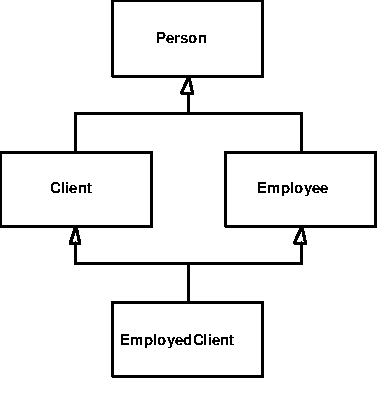
\includegraphics{Abstraction/EmployedClient.pdf}
    \end{center}  
    \caption{An employed client is a client and an employee.
             \label{figEmployedClient}} 
  \end{figure}
%\end{latexonly}  

Indeed, the {\em is a} test is satisfied along 
both legs, an \verb+EmployedClient+ is an \verb+Employee+ and 
{\em is a} client. Hence, if somebody expects an \verb+Employee+

\noindent{\small \begin{verbatim}
double restructureSalary(Employee& employee)
{
  ...
}
\end{verbatim}}  

\noindent
you should be able to pass any \verb+Person+ which {\em is an}
\verb+Employee+, i.e.\ an instance of \verb+Employee+ or an
instance of the \verb+EmployedClient+ class.

Similarly, if somebody expects a \verb+Client+

\noindent{\small \begin{verbatim}
void debitMonthlyServiceFees(Client& client)
{
  ...
}
\end{verbatim}}  


Unlike Java, C++ does support multiple inheritance 
of classes, i.e.\ a class can be a subclass of more than one class.

%--------------------------------------------------------------------

\subsection{Simplistic Multiple Inheritance and its Problems}

Let us simplistically define a \verb+Client+ class as follows:

\noindent {\small \input{Abstraction/Programs/Client1.h}}

We provide a trivial implementation of this class in:

\noindent {\small \input{Abstraction/Programs/Client1.cpp}}

Now we are in a position to define an \verb+EmployedClient+ class.
Let us simply define a join class which adds no new services above
those inherited from the \verb+Employee+ and \verb+Client+
superclasses:

\noindent {\small \input{Abstraction/Programs/EmployedClient1.h}}

We provide a trivial implementation of this class in:

\noindent {\small \input{Abstraction/Programs/EmployedClient1.cpp}}

Now, when we use instances of the the \verb+EmployedClient+ class, 
we can directly ask them for their salary or their account:

\noindent {\small \input{Abstraction/Programs/MultInheritance1.cpp}}

There are, however, a number of severe problems: 
\begin{itemize}
  \item Firstly, our employed client is an \verb+Employee+, but somehow
        he/she is not a Person??? This manifests itself in that we
        are able to have an \verb+Employee+ pointer point to an employed client
        (he/she is, after all, an \verb+Employee+), but when we try and
        assign a \verb+Person+ pointer to the employed client we are told
        that it is not a \verb+Person+.
  \item Secondly, though we can make use of the inherited \verb+salary()+
        and \verb+account()+ services we somehow do not inherit \verb+name()+
        and \verb+idNo()+.
\end{itemize}

But things get even stranger. Let us define anothe subclass of \verb+Employee+,
a \verb+Manager+ class:

\noindent {\small \input{Abstraction/Programs/Manager.h}}

with implementation

\noindent {\small \input{Abstraction/Programs/Manager.cpp}}

If we create an instance of this class then we can assign a \verb+Person+ 
pointer to it and we can request the \verb+name()+ and \verb+idNo()+
services. So why could we not do it for \verb+Employee+s.

The answer lies in the way we derived \verb+Employee1+ and \verb+Client1+
from \verb+Person+. The default thing C++ does is, from an object-oriented 
perspective, incorrect.

Recall that when we instantiate a class, all its superclasses are 
instantiated too. So, when we create an \verb+Employee+ we create a 
\verb+Person+, and similarly, creating a \verb+Manager_+creates an 
\verb+Employee+ which creates a \verb+Person+. So far, no problem -- 
and indeed, the \verb+Manager+ class behaved correctly.

Lets look wha\t happens in the \verb+EmployedClient+ case. Creating an
\verb+EmployedClient+ creates both, an \verb+Employee+ as well as a
\verb+Client+. Each of these, in turn, creates a \verb+Person+. Our
\verb+EmployedClient+ class {\em is} thus two persons and not a single 
person. That is why we could not assign a \verb+Person+ pointer to the
\verb+EmployedClient+. Also, when we requested the \verb+name()+ service
the compiler did not know which person's name he/she/it should choose.

This is, of course, nonsensical. An employed client is of course 
an employee, as well as a client and a single person. Any other
scenario does not make logical sense. This is, however, not the
way it is seen by default in C++. So how do we fix it?

%--------------------------------------------------------------------

\subsection{Virtual Specialization}

We want to specify that every client and every employee {\em is a single}
\verb+Person+. This is specified by inserting the \verb+virtual+ keyword
in the inheritance link. This has to be done when deriving both, \verb+Client+
class

\noindent {\small \input{Abstraction/Programs/Client.h}}

and the employee class

\noindent {\small \input{Abstraction/Programs/Employee.h}}

from the verb+Person+ class. The implementations of these classes are identical
to the implementations of the \verb+Employee1+ and \verb+Client+ classes
shown above. 

The header of the \verb+EmployedClient+ class could remain as above, though
we do change the inheritance links to virtual for reasons discussed below.

\noindent {\small \input{Abstraction/Programs/EmployedClient.h}}

We have to modify the implementation of the constructor, though. Not only
do we have to specify how the direct subclasses are isntantiated, but we
also have to specify how the one and only instance of the \verb+Person+
class is created:

\noindent {\small \input{Abstraction/Programs/EmployedClient.cpp}}

Now things do behave correctly as illustrated in the code below:

\noindent {\small \input{Abstraction/Programs/MultInheritance.cpp}}

Note that we had to realize the potential problem early, i.e.\ when we 
defined the \verb+Client+ and \verb+Employee+ subclasses -- not when we 
did our multiple inheritance thing. At that stage it may not have dawned 
on us that we will one day have employed clients which are both employees 
and clients. One ust has to have this mystical feeling.

No, more seriously, specialization should, from an object-oriented 
perspective, allways be \verb+virtual+. If you define a non-virtual 
subclass, then you are specifying what is known in UML as a 
\verb+{disjoint}+ constraint -- i.e.\ that all subclasses of that class
may not multply inherit from any classes within that particular class 
hierarchy.

